\section{CAP teorien}
\begin{figure}[H]
    \centering
    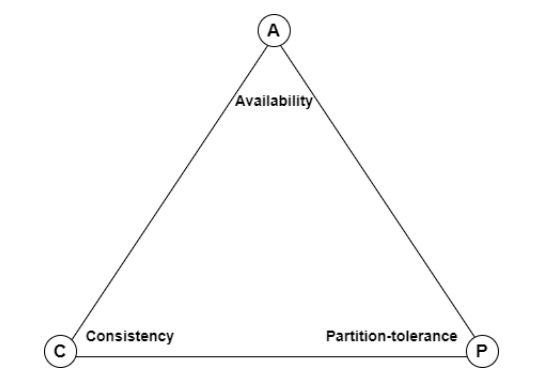
\includegraphics[scale=0.65]{cap.png}
    \caption{CAP teorien}
    \label{fig::cap}
\end{figure}

I snakken om databaser anses CAP-theorem som værende en af de fundamentale teorier, og er særligt brugt i beslutningsprocessen om hvilke databaser der skal tages i brug. Teorien blev præsenteret i 2000 af Eric Brewer\cite{capibm} der viser, at et distribueret system kun kan opfylde to ud af tre garantier. Garantierne er illustreret i figur \ref{fig::cap}, og lyder:
\begin{itemize}
    \item C: Konsistent: Hvert read-request modtager altid et svar med det nyeste data eller en fejlmeddelelse.
    \item A: Tilgængelighed: Hvert request modtager et validt svar, uden garanti for at det er det seneste data.
    \item P: Partitionstolerance: Systemet skal kunne fortsætte med at fungere på trods af kommunikation sammenbrud mellem noderne i systemet.
\end{itemize}
Ifølge logikken bag teorien, kan et databasesystem ikke opfylde alle tre garantier, hvilket medfører at en database må gå på kompromis med en garanti. En database kan derfor enten være AC, AP eller CP. Hver har sine fordele og ulemper, som bør tages til eftertanke. CAP teorien bliver ofte refereret til sammen med ACID og BASE, som er databasemodeller der fundamentalt betegner hvordan en database håndterer begrænsningerne af CAP. Eksempelvis vil SQL databaser og graph databaser ifølge teorien som udgangspunkt opfylde tilgængelighed og konsistent garantierne, hvilket gør dem ACID kompatible. Dermed er dataen højt tilgængelig og sikret at det er det nyeste data. Ligeledes betyder dette at partitionstolerance ikke kan opfyldes.